\documentclass[mathserif]{beamer}

\usepackage{thesis}
\usepackage{pdfpages}

\title[Sampling from Probabilistic Submodular Models]
{Sampling from Probabilistic Submodular Models}

\author[Alkis Gotovos]{}


\newcommand{\btheta}{\*\theta}
\newcommand{\bu}{\*u}
\newcommand{\bw}{\*w}
\newcommand{\bv}{\*v}
\newcommand{\defeq}{\vcentcolon=}

\newcommand{\tab}[2]{%
\makebox[#1\linewidth][l]{#2}%
}

\begin{document}

\setbeamertemplate{background canvas}{}
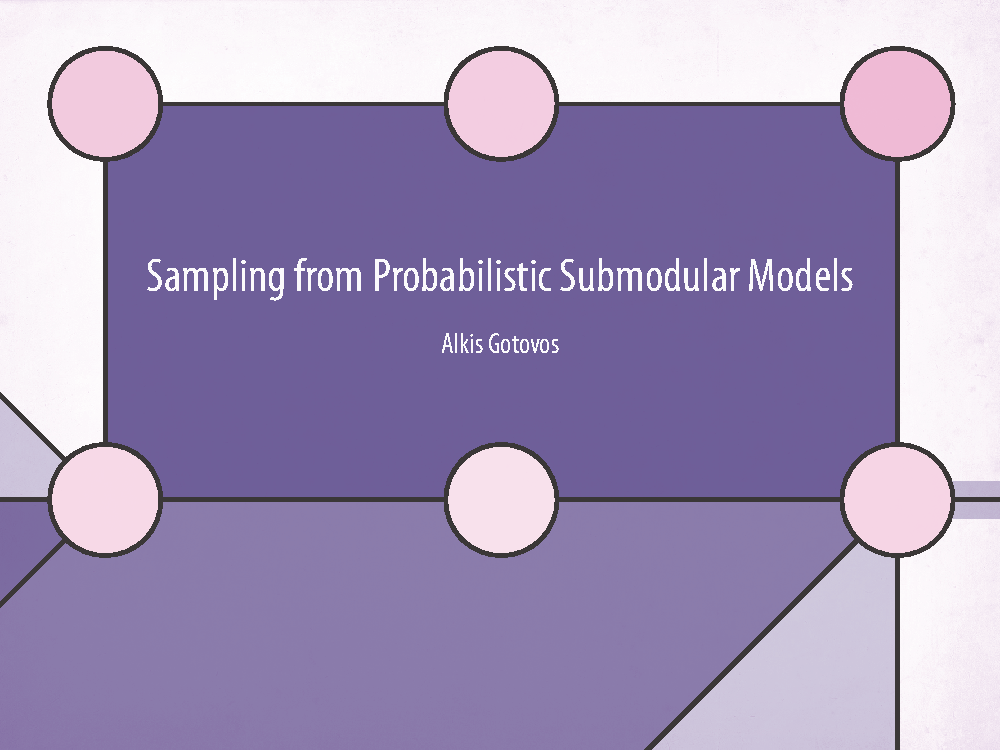
\includepdf[pages={1}]{title/title.pdf}
\setbeamertemplate{background canvas}{
\includegraphics[width=\paperwidth]{figures/bg_no_line.png}}


\begin{frame}{The Cancer Genome Atlas}
\vspace{0.5em}
\centering
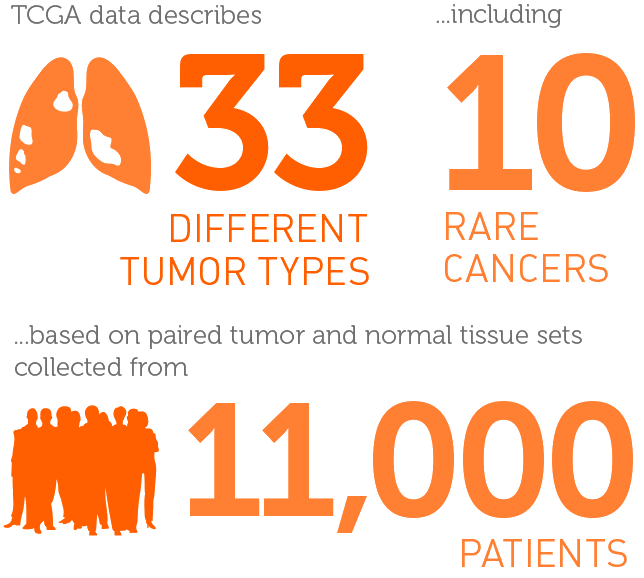
\includegraphics[width=2.5in]{figures/tcga.png}\\[-0.3em]
\hspace{12em}\qsource{cancergenome.nih.gov}
\end{frame}

\begin{frame}{The Cancer Genome Atlas}
\vspace{0.3em}
\centering
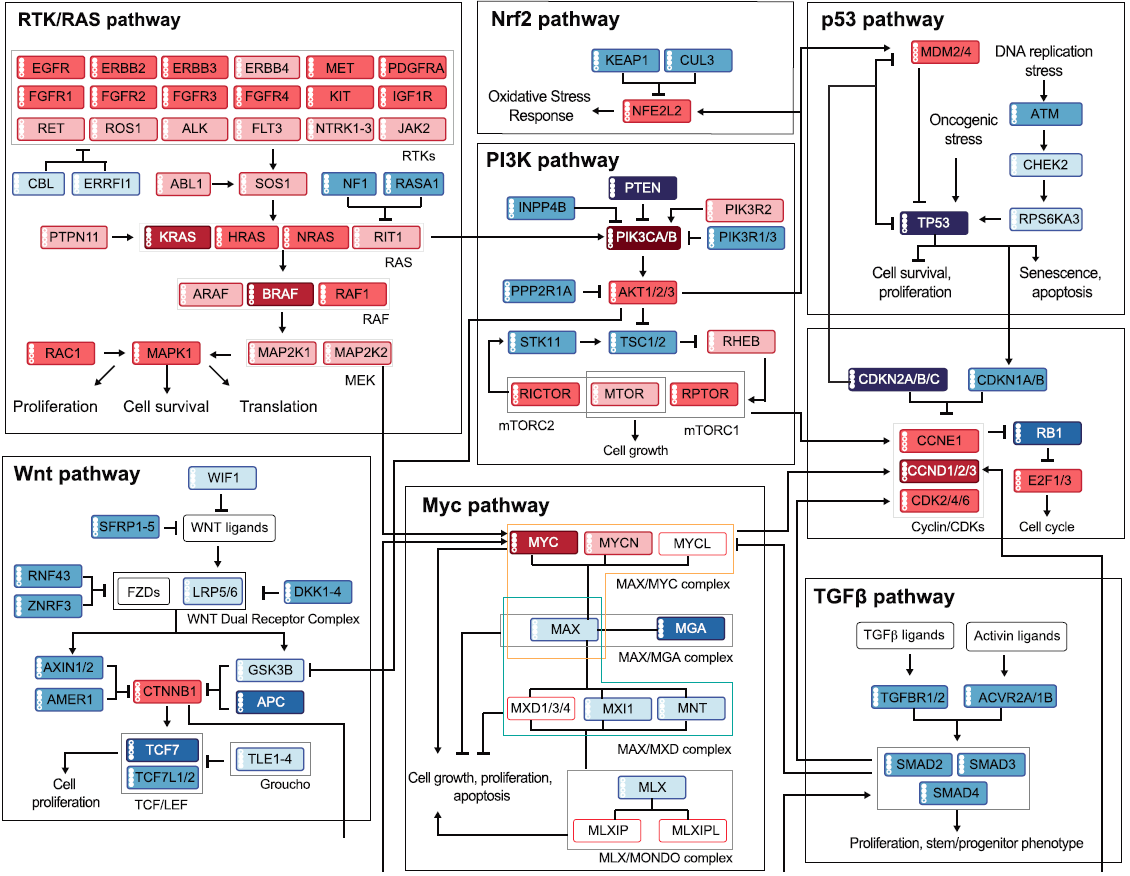
\includegraphics[width=3.85in]{figures/pathways_new.png}\\[-0.7em]
\hspace{22em}\qsource{Schultz et al., 2018}
\end{frame}

\begin{frame}{Modeling Interactions between Gene Mutations}
\centering
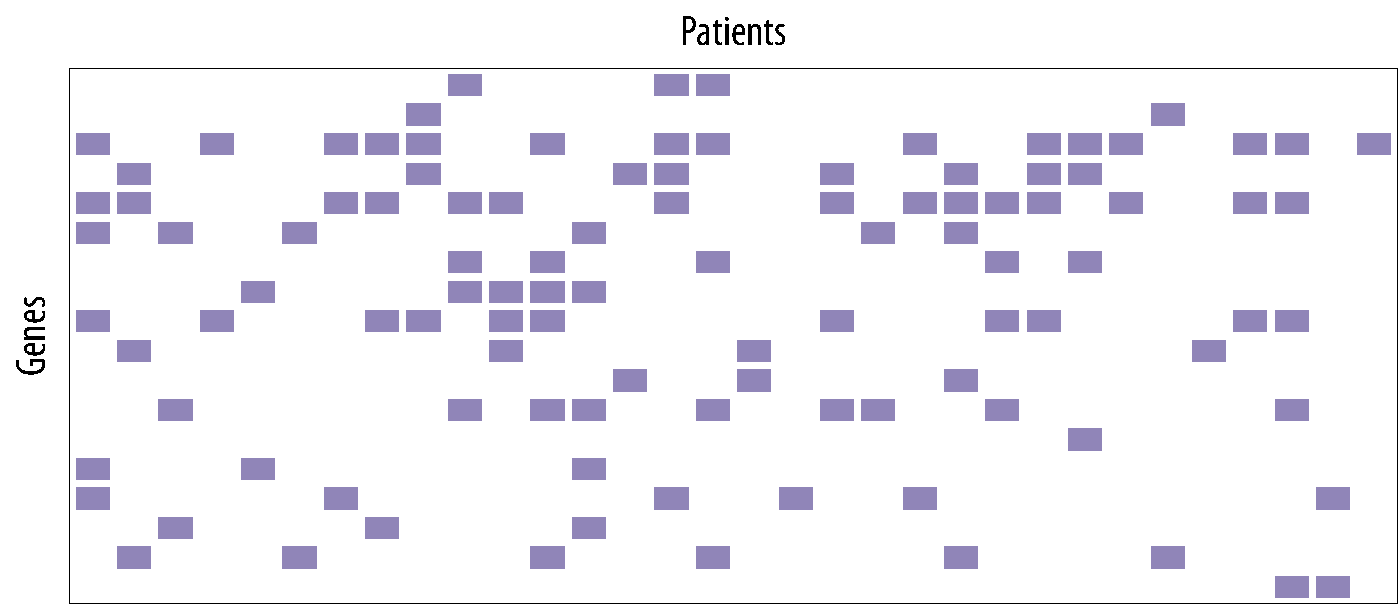
\includegraphics[width=3.7in]{figures/example1.pdf}
\end{frame}

\begin{frame}{Modeling Interactions between Gene Mutations}
\centering
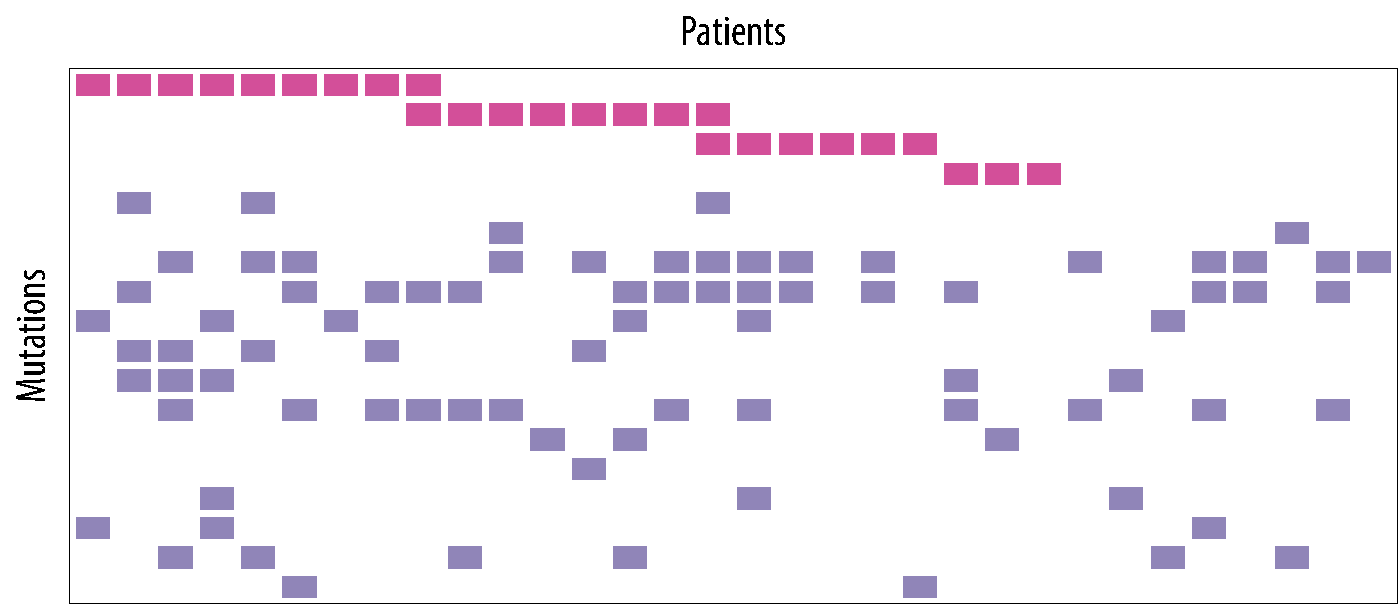
\includegraphics[width=3.7in]{figures/example1_rep.pdf}
\end{frame}

\begin{frame}{Modeling Interactions between Gene Mutations}
\centering
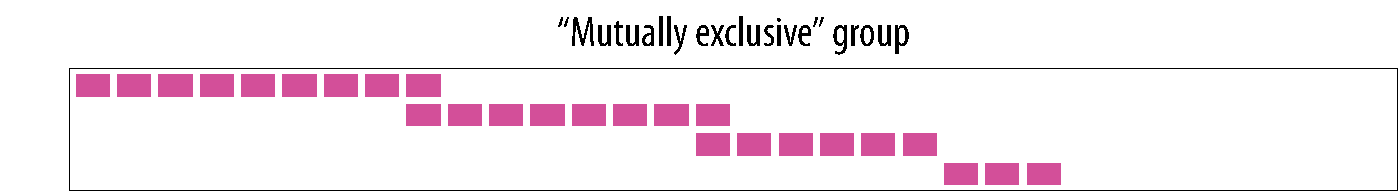
\includegraphics[width=3.7in]{figures/example1_rep_group.pdf}

\vspace{3em}

\begin{itemize}
\item \tab{0.4}{Discrete optimization \hspace{0.3em} 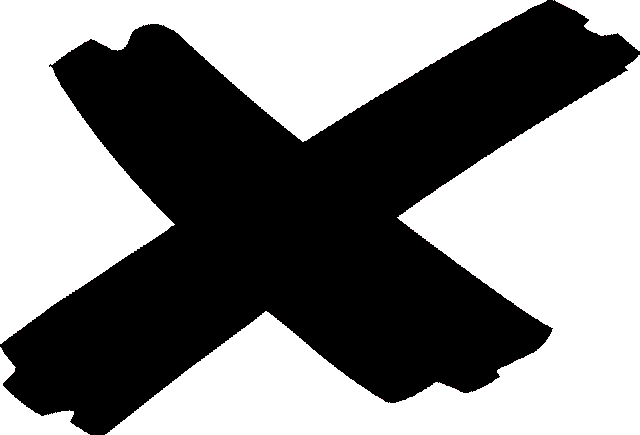
\includegraphics[width=0.13in]{figures/cross_mark.png}} \tab{0.15}{$\longrightarrow$} probabilistic models \hspace{0.3em} 
\includegraphics[width=0.13in]{figures/check_mark.png}
\vspace{0.7em}
\item \tab{0.4}{Classic pairwise models \hspace{0.3em} 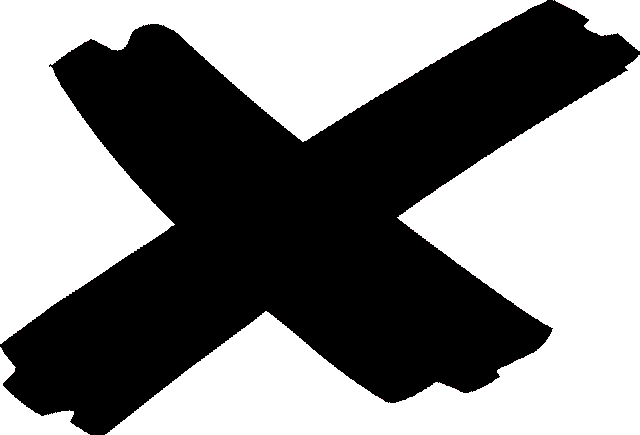
\includegraphics[width=0.13in]{figures/cross_mark.png}} \tab{0.15}{$\longrightarrow$} higher-order interactions \hspace{0.3em} 
\includegraphics[width=0.13in]{figures/check_mark.png}
\vspace{0.7em}
\item \tab{0.4}{Deep nets \hspace{0.3em} 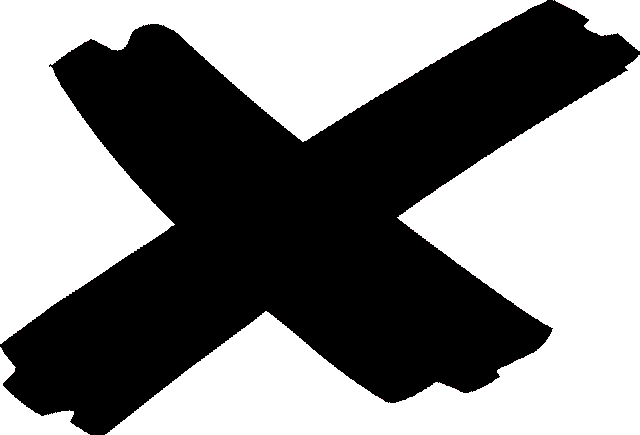
\includegraphics[width=0.13in]{figures/cross_mark.png}} \tab{0.15}{$\longrightarrow$} structured prior assumptions \hspace{0.3em} 
\includegraphics[width=0.13in]{figures/check_mark.png}
\end{itemize}
\end{frame}

\begin{frame}{Probabilistic Submodular Models}

\begin{center}
Distributions over subsets of $V = \{1,\ldots,n\}$

\vspace{0.8em}
\qboxa{
$p(S; \btheta) = \displaystyle\frac{1}{Z(\btheta)}\exp \big( F(S; \btheta) \big)$
}
\end{center}
\vspace{2em}

\begin{columns}
\begin{column}{0.54\textwidth}
\begin{itemize}
\item $F : 2^V \to \mathbb{R}\ $ is sub- or supermodular
\item $Z\ $ is the normalizer
\item $\btheta\ $ is a parameter vector
\end{itemize}
\end{column}
\begin{column}{0.39\textwidth}
\begin{itemize}
\item Ising model (log-supermodular)
\item DPP (log-submodular)
\end{itemize}
\end{column}
\end{columns}

\end{frame}

\begin{frame}{Inference}
\begin{center}
Distributions over subsets of $V = \{1,\ldots,n\}$

\vspace{0.8em}
\qboxa{
$p(S; \btheta) = \displaystyle\frac{1}{Z(\btheta)}\exp \big( F(S; \btheta) \big)$
}
\end{center}
\vspace{2em}

Fundamental tasks
\vspace{0.5em}
\hspace{11em}\tikzmark{right}
\begin{itemize}
\item Compute marginals $\ \mathbb{P}(a \in S \mid \{b, c\} \subseteq S)$ \tikzmark{i2}
\item Compute $\ Z$ \tikzmark{i3}
\item Learn $\btheta$ from data
\end{itemize}

\begin{tikzpicture}[overlay, remember picture]
\node[anchor=base] (a) at (pic cs:i2) {\vphantom{h}}; % push the mark to the top of the line (ie including ascenders)
\node[anchor=base] (b) at (pic cs:i3) {\vphantom{g}}; % push the mark to the bottom of the line (ie including descenders)
\draw [decoration={brace,amplitude=0.5em},decorate,thick,col2]
 (a.north -| {pic cs:right}) -- (b.south -| {pic cs:right});
\node [text=col2,xshift=10.4em] (t) at ($(a)!0.5!(b)$) {\#P-hard in general};
\end{tikzpicture}

\end{frame}

\begin{frame}{Inference}
\vspace{0.5em}

\begin{minipage}{\textwidth}
\begin{columns}[c]
\column{0.36\textwidth}
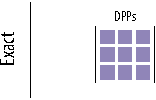
\includegraphics[height=0.7in]{figures/inf_dpp.pdf}
\column{0.57\textwidth}
\begin{itemize}
\item Tractable only for limited subclasses
\vspace{0.3em}
\item \#P-hard even for Ising models
\end{itemize}
\end{columns}
\end{minipage}

%\uncover<2->{
\vspace{2em}
\begin{minipage}{\textwidth}
\begin{columns}[c]
\column{0.36\textwidth}
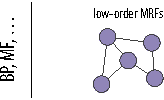
\includegraphics[height=0.7in]{figures/inf_mrf.pdf}
\column{0.57\textwidth}
\begin{itemize}
\item Extensively studied model class
\vspace{0.3em}
\item Complexity exponential in model order
\end{itemize}
\end{columns}
\end{minipage}
%}

%\uncover<3->{
\vspace{2em}
\begin{minipage}{\textwidth}
\begin{columns}[c]
\column{0.36\textwidth}
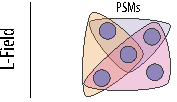
\includegraphics[height=0.7in]{figures/inf_psm.pdf}
\column{0.57\textwidth}
\begin{itemize}
\item Variational approach for general PSMs\\
\qcitea{Djolonga and Krause, 2014; Djolonga and Krause, 2015}
\end{itemize}
\end{columns}
\end{minipage}
%}
\end{frame}

\begin{frame}{Thesis Topic}
\vspace{1em}
\centering
\only<1>{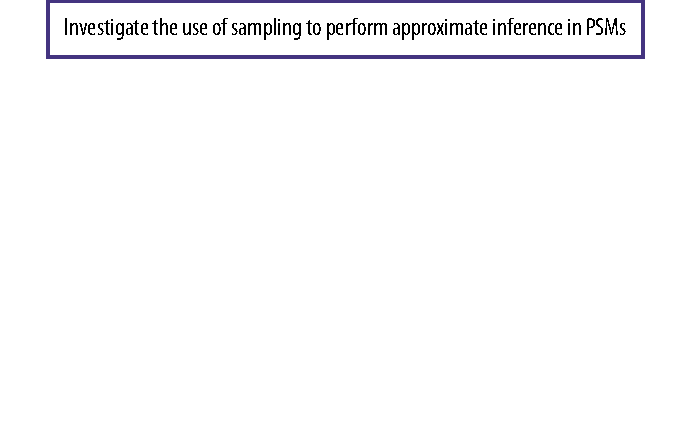
\includegraphics[width=\textwidth]{figures/chapters_topic.pdf}}%
\only<2>{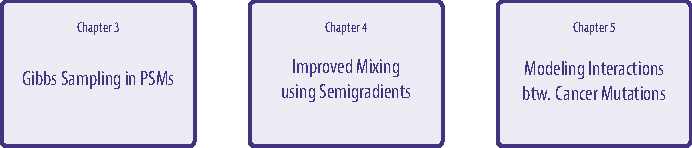
\includegraphics[width=\textwidth]{figures/chapters.pdf}}
\end{frame}

\begin{frame}{Gibbs Sampling in PSMs}
\vspace{1em}
\centering
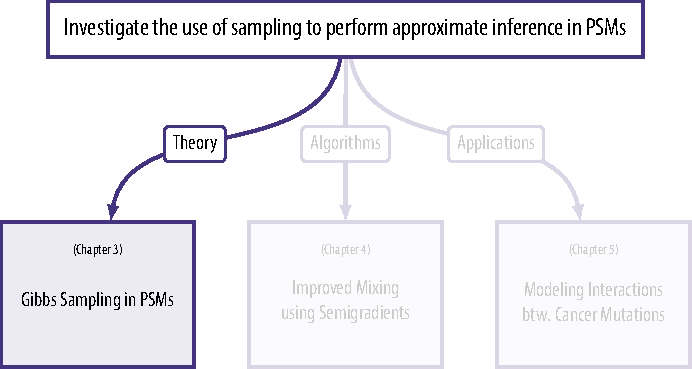
\includegraphics[width=\textwidth]{figures/chapters1.pdf}
\end{frame}

\begin{frame}{Sampling}
\begin{itemize}
\item Ground set $\ V = \{1,\ldots,n\}$
\item State space $\ \Omega = 2^V$
\item Transition matrix $\ P : \Omega \times \Omega \to \mathbb{R}$
\end{itemize}

%\vspace{1em}
\begin{center}
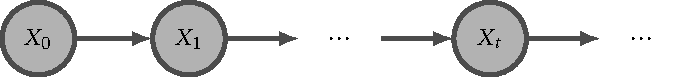
\includegraphics[width=3.3in]{figures/markov.pdf}
\end{center}

\vspace{1em}
Distance from stationarity $\ \ d(t) \defeq \max \left\{\|\mathbb{P}_{X_t} - p\|_{\textrm{tv}} \mid X_0 \in \Omega\right\}$\\[1.5em]
Under mild conditions, $\ \ d(t) \xrightarrow{\ t\,\rightarrow\,\infty\ } 0\ \ \ \ $ {\color{col2} how fast?}\\[1.6em]
Mixing time $\ \ t_{\textrm{mix}}(\epsilon) = \min \left\{t \mid d(t) \leq \epsilon \right\}$
\end{frame}

\begin{frame}{The Gibbs Sampler}
\vspace{1em}
\centering
\only<1>{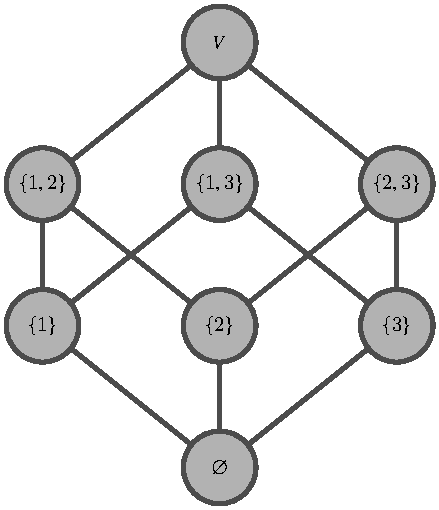
\includegraphics[width=2.5in]{figures/lattice_gibbs_0.pdf}}%
\only<2>{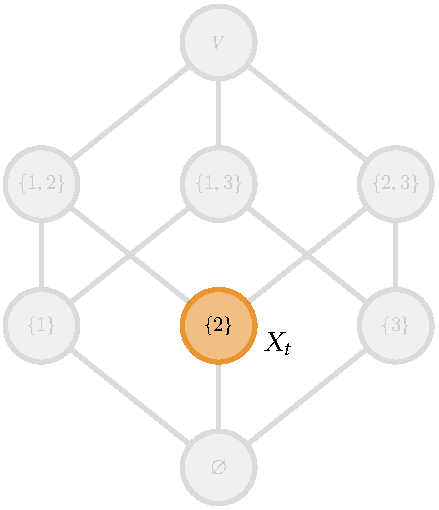
\includegraphics[width=2.5in]{figures/lattice_gibbs_1.pdf}}%
\only<3>{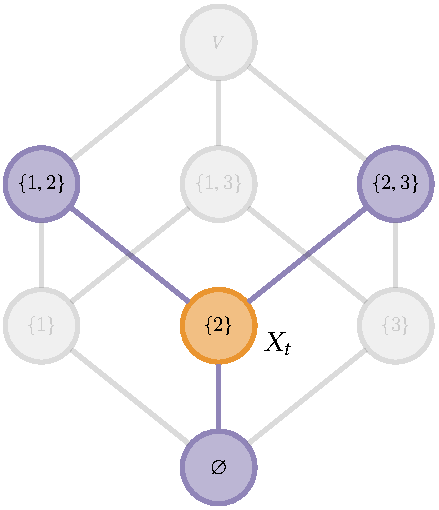
\includegraphics[width=2.5in]{figures/lattice_gibbs_2.pdf}}%
\end{frame}

\begin{frame}{Improved Mixing using Semigradients}
\centering
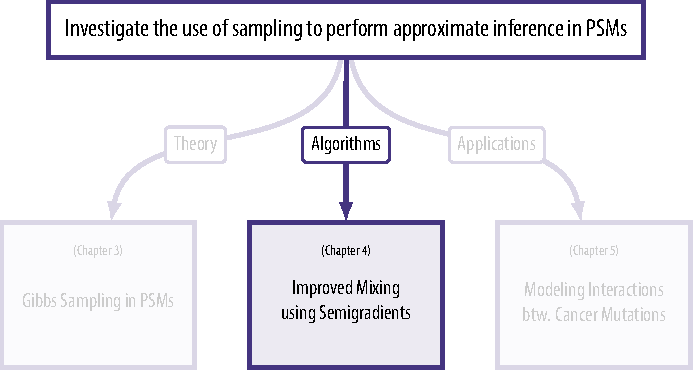
\includegraphics[width=\textwidth]{figures/chapters2.pdf}
\end{frame}

\begin{frame}{Modeling Interactions between Cancer Mutations}
\centering
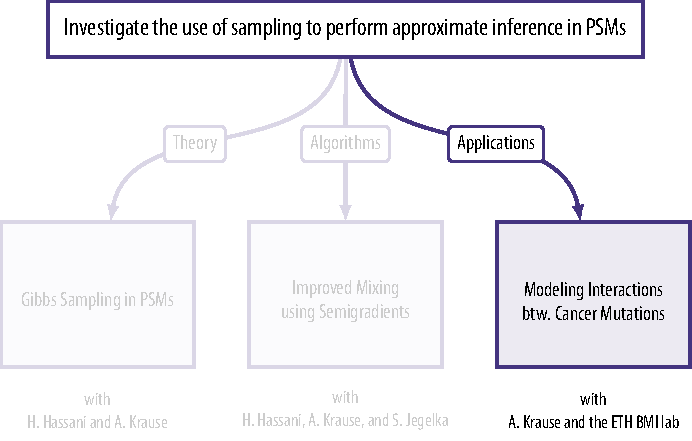
\includegraphics[width=\textwidth]{figures/chapters3.pdf}
\end{frame}

\end{document}
